\documentclass[11pt]{article}

% ══════════════════════════════════════════════════════════════════════════════
%  PACKAGES
% ══════════════════════════════════════════════════════════════════════════════
\usepackage[T1]{fontenc}
\usepackage[utf8]{inputenc}
\usepackage{amsmath,amssymb,amsfonts,amsthm}
\usepackage{graphicx}
\usepackage{bm}
\usepackage{siunitx}
\usepackage{geometry}
\usepackage[colorlinks=true,linkcolor=black,citecolor=blue,urlcolor=blue]{hyperref}
\usepackage[noabbrev,nameinlink]{cleveref}
\usepackage{xcolor}
\usepackage{booktabs}
\usepackage{enumitem}
\usepackage{listings}

\geometry{margin=1in}

% Theorem environments
\theoremstyle{definition}
\newtheorem{definition}{Definition}[section]
\newtheorem{assumption}{Assumption}[section]

% Code style
\lstdefinestyle{pythonblock}{%
  backgroundcolor=\color{black!95},
  basicstyle=\ttfamily\small\color{white},
  frame=single,
  numbers=left,
  numberstyle=\tiny\color{gray},
  breaklines=true,
  keywordstyle=\color{cyan},
  commentstyle=\color{gray},
  stringstyle=\color{yellow},
  showstringspaces=false
}

% ══════════════════════════════════════════════════════════════════════════════
%  TITLE
% ══════════════════════════════════════════════════════════════════════════════
\title{One-Dimensional Slug-Flow Model for Self-Starting Siphons:\\
       Theory, Bounds, and Computation\\[0.5em]
       \rule{\textwidth}{0.4pt}\\[0.5em]
       \large IYPT 2026 Problem \#1}
\author{Stylianos Raptopouos}
\date{24/11/2025}

\begin{document}
\maketitle

% ══════════════════════════════════════════════════════════════════════════════
%  ABSTRACT
% ══════════════════════════════════════════════════════════════════════════════
\begin{abstract}
Self-starting siphons prime spontaneously when partially immersed, without external suction. 
This document develops a one-dimensional slug-flow model that connects geometric and physical 
parameters to observable outcomes---priming success, filling time, and draining rate---for 
IYPT 2026 Problem~\#1.

The model yields three main results: (i)~an analytical upper bound $h_{\max}$ for the maximum 
climb height, expressed in closed form for piecewise-linear pipe geometries; (ii)~a geometric 
priming criterion $h_{\max} > h_{\text{crest}}$ that screens infeasible designs without 
numerical integration; and (iii)~explicit ordinary differential equations for the full 
time evolution, incorporating Churchill friction and minor losses.

The deliberate simplicity of treating the liquid as a rigid slug enables rapid parameter 
exploration (seconds per case) and makes the physics transparent. Discrepancies between 
model predictions and experiments or CFD directly highlight where additional mechanisms---such 
as three-dimensional flow structure, air entrainment, or column separation---become important.
\end{abstract}

\tableofcontents
\newpage

% ══════════════════════════════════════════════════════════════════════════════
%  SECTION 1: INTRODUCTION
% ══════════════════════════════════════════════════════════════════════════════
\section{Introduction}
\label{sec:intro}

\subsection{The IYPT problem}

The International Young Physicists' Tournament (IYPT) 2026 Problem~\#1 states:
\begin{quote}
\emph{``A self-starting siphon can be made using a piece of rigid tubing bent into a specific 
shape. When the siphon is partially immersed in water, it begins siphoning water without the 
need for initial suction. Investigate how the relevant parameters, such as the geometry, 
affect the siphoning process.''}
\end{quote}

This open-ended question requires identifying the controlling parameters, establishing 
quantitative relationships between parameters and outcomes, understanding underlying 
mechanisms and their limits, and exploring failure regimes.

\subsection{Physical mechanism}

Self-starting siphons differ from conventional inverted-U siphons in that they do not require 
pre-filling or an externally imposed pressure difference. Instead, the geometry is arranged 
so that an initial drop converts gravitational potential energy into kinetic energy, and the 
resulting momentum carries a water slug over a crest before friction and gravity bring it to 
rest. Once the crest is crossed, standard siphon action continues until the driving head is 
exhausted. Classical discussions of siphon behaviour and the role of atmospheric pressure and 
cohesion can be found in Potter and Barnes~\cite{potter_barnes} and Jumper and Stanchev~\cite{jumper_stanchev}.

The key insight is that in a properly designed self-starting geometry, the driving head 
$h_c(t) - h(L(t))$ (container surface minus front elevation) remains positive for an extended 
portion of the climb, allowing the slug to build momentum. By contrast, in a simple inverted-U 
siphon the driving head vanishes at the crest after the initial drop, so no momentum advantage 
accumulates.

\subsection{Document structure}

Section~\ref{sec:setup} establishes the geometry and notation. Section~\ref{sec:conservation} 
derives volume conservation and the container drawdown relation. Section~\ref{sec:momentum} 
presents the unified momentum derivation from first principles. Section~\ref{sec:filling} 
assembles the complete filling-phase dynamics. Section~\ref{sec:bounds} develops the 
analytical climb bound and geometric priming criterion. Section~\ref{sec:draining} treats 
the draining phase. Section~\ref{sec:validity} discusses validity limits. 
Section~\ref{sec:computation} presents the computational implementation, and 
Section~\ref{sec:conclusions} summarises the model.

% ══════════════════════════════════════════════════════════════════════════════
%  SECTION 2: PROBLEM SETUP
% ══════════════════════════════════════════════════════════════════════════════
\section{Problem Setup: Geometry and Notation}
\label{sec:setup}

\subsection{Coordinate system}

We work in a two-dimensional vertical plane with coordinates $(x,h)$, where $x$ is horizontal 
(increasing rightward) and $h$ is vertical (increasing upward). The vertical datum is chosen 
so that $h = 0$ at the container base.

\subsection{Pipe geometry: five nodes and four segments}

The pipe centreline is defined by five nodes
\[
  A = (x_0, h_0), \quad
  B = (x_1, h_1), \quad
  C = (x_2, h_2), \quad
  D = (x_3, h_3), \quad
  E = (x_4, h_4),
\]
connected by four straight segments. Node $A$ is at the pipe inlet (container wall), and 
node $E$ is at the outlet. By convention, $D$ is the crest (highest point on the path).

\begin{figure}[ht]
  \centering
  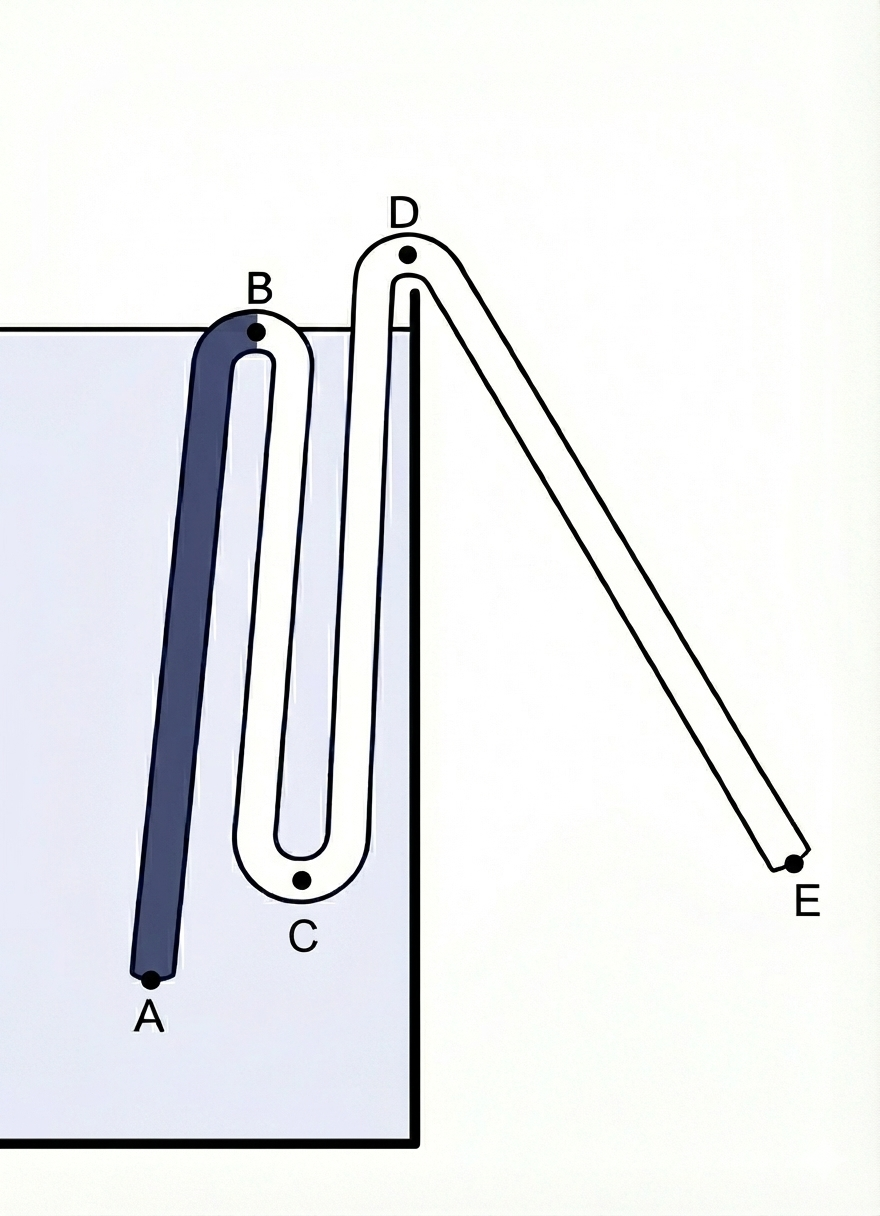
\includegraphics[width=0.6\textwidth]{siphon_model}
  \caption{Schematic of the self-starting siphon geometry and node labelling.}
  \label{fig:siphon-geometry}
\end{figure}

The length of each segment is
\[
  L_i = \sqrt{(x_i - x_{i-1})^2 + (h_i - h_{i-1})^2}, \qquad i = 1,2,3,4,
\]
and the total pipe length is $L_{\max} = L_1 + L_2 + L_3 + L_4$.

\subsection{Arclength coordinate and centreline elevation}

We parameterise the pipe centreline by arclength $L$, measured from the inlet:
\[
  L = 0 \text{ at } A, \quad
  L = L_1 \text{ at } B, \quad
  L = L_1 + L_2 \text{ at } C, \quad
  L = L_1 + L_2 + L_3 \text{ at } D, \quad
  L = L_{\max} \text{ at } E.
\]
It is convenient to define cumulative lengths
\[
  S_0 = 0, \quad S_1 = L_1, \quad S_2 = L_1 + L_2, \quad S_3 = L_1 + L_2 + L_3, \quad S_4 = L_{\max}.
\]

Since each segment is straight, the centreline elevation $h(L)$ is piecewise linear. On 
segment $i$ (for $L \in [S_{i-1}, S_i]$) we write
\begin{equation}
  h(L) = c_i + s_i L,
  \label{eq:hL-affine}
\end{equation}
where the slope is
\begin{equation}
  s_i = \frac{h_i - h_{i-1}}{L_i} = \sin\theta_i
  \label{eq:slope}
\end{equation}
(with $\theta_i$ the inclination angle to horizontal) and the intercept is
\begin{equation}
  c_i = h_{i-1} - s_i S_{i-1}.
  \label{eq:intercept}
\end{equation}
Only the vertical projection of each leg enters the dynamics---horizontal extent affects 
segment length but not the gravitational driving force.

\subsection{State variables}

During the \emph{filling phase}, the pipe is partially full. The state is characterised by:
\begin{itemize}[nosep]
  \item $L(t)$: the wetted length (arclength from inlet to the advancing front),
  \item $h_c(t)$: the container free-surface elevation.
\end{itemize}
The front velocity is $v(t) = \dot{L}(t)$, and the front elevation is $h(L(t))$.

During the \emph{draining phase}, the pipe is completely full ($L = L_{\max}$), and the 
state becomes $(h_c(t), v(t))$ where $v(t)$ is now the mean pipe velocity.

\subsection{Container and pipe parameters}

\begin{center}
\renewcommand{\arraystretch}{1.2}
\begin{tabular}{lll}
\toprule
Symbol & Units & Description \\
\midrule
$A_0$ & m$^2$ & Effective container cross-sectional area \\
$A$ & m$^2$ & Pipe cross-sectional area, $A = \pi D^2/4$ \\
$D$ & m & Pipe inner diameter \\
$\rho$ & kg/m$^3$ & Fluid density \\
$\mu$ & Pa$\cdot$s & Dynamic viscosity \\
$\varepsilon/D$ & --- & Relative pipe roughness \\
$\sum K_i$ & --- & Total minor-loss coefficient \\
\bottomrule
\end{tabular}
\end{center}

The container is assumed large enough that the free surface remains quasi-hydrostatic 
(velocities at the surface are negligible compared to pipe velocities).

% ══════════════════════════════════════════════════════════════════════════════
%  SECTION 3: MASS CONSERVATION
% ══════════════════════════════════════════════════════════════════════════════
\section{Mass Conservation and Container Drawdown}
\label{sec:conservation}

\subsection{Volume balance during filling}

During the filling phase, no water has left the outlet, so the total volume in the 
container--pipe system is conserved:
\begin{equation}
  V_{\text{cont}}(t) + V_{\text{pipe}}(t) = V_{\text{tot}} = \text{constant}.
  \label{eq:vol-conserve}
\end{equation}
With $V_{\text{cont}}(t) = A_0 h_c(t)$ and $V_{\text{pipe}}(t) = A L(t)$, this becomes
\[
  A_0 h_c(t) + A L(t) = A_0 h_c(0) + A L(0).
\]

\subsection{Initial conditions}
\label{sec:ICs}

We define $t = 0$ as the instant when the dynamical filling phase begins. Two common 
preparation procedures lead to the same initial state:
\begin{enumerate}[nosep]
  \item \emph{Pre-fill}: slowly fill the container until the water surface reaches node $B$, 
        fully wetting segment $AB$.
  \item \emph{Dip}: submerge the inlet until the internal level reaches $B$, then position 
        the device.
\end{enumerate}
In both cases, the preparatory motion is slow, so at $t = 0$ the front has just arrived at 
$B$ with negligible velocity. The initial conditions are therefore
\begin{equation}
  \boxed{L(0) = L_1, \qquad \dot{L}(0) = 0, \qquad h_c(0) = h_0.}
  \label{eq:ICs}
\end{equation}
The total volume is $V_{\text{tot}} = A_0 h_0 + A L_1$.

\subsection{Container level as a function of wetted length}

Solving \eqref{eq:vol-conserve} for $h_c$ in terms of $L$ gives the key kinematic relation:
\begin{equation}
  \boxed{h_c(L) = h_0 - \frac{A}{A_0}(L - L_1).}
  \label{eq:hc-of-L}
\end{equation}
The container level decreases linearly as the front advances. The ratio $A/A_0$ controls 
how quickly the driving head diminishes: large containers ($A_0 \gg A$) experience minimal 
drawdown, while small containers can lose driving head rapidly.

\textbf{Remark on generalisation.} For complex internal pipe layouts where the number of 
pipe legs intersected by a horizontal slice varies with elevation, the effective area 
$A_{\text{eff}}(\eta)$ becomes height-dependent. The volume map is then 
$V_{\text{cont}} = \int_0^{h_c} A_{\text{eff}}(\eta)\,d\eta$, and $h_c(L)$ must be obtained 
from an implicit relation. In this document, we adopt the constant-$A_0$ approximation, 
which is accurate when the pipe diameter is small compared to the container radius.

% ══════════════════════════════════════════════════════════════════════════════
%  SECTION 4: MOMENTUM BALANCE
% ══════════════════════════════════════════════════════════════════════════════
\section{Momentum Balance: Derivation from First Principles}
\label{sec:momentum}

This section derives the equation of motion for the water slug by integrating pressure and 
gravitational forces along the pipe. The derivation is presented once, in full, to establish 
the result rigorously.

\subsection{Setup}

Consider the water in the pipe as a slug of length $L(t)$, cross-sectional area $A$, and 
uniform mean velocity $v(t) = \dot{L}(t)$. Introduce a local arclength coordinate $\xi$ 
measured from the inlet, so $\xi$ runs from $0$ (at $A$) to $L(t)$ (at the front).

At position $\xi$, the centreline elevation is $h(\xi)$ and the pressure is $p(\xi, t)$.

\subsection{Forces on a fluid slice}

Consider a thin slice between $\xi$ and $\xi + d\xi$:
\begin{itemize}[nosep]
  \item Mass: $dm = \rho A\,d\xi$
  \item Upstream pressure force (in direction of motion): $+p(\xi, t) A$
  \item Downstream pressure force: $-p(\xi + d\xi, t) A$
  \item Gravitational component along pipe: $-\rho g A \dfrac{dh}{d\xi}\,d\xi$
\end{itemize}
The net tangential force on the slice is
\[
  dF = -A \frac{\partial p}{\partial \xi}\,d\xi - \rho g A \frac{dh}{d\xi}\,d\xi.
\]

\subsection{Integration along the slug}

Integrating from $\xi = 0$ to $\xi = L$ gives the total force:
\begin{align}
  F_{\text{net}} &= -A \int_0^L \frac{\partial p}{\partial \xi}\,d\xi 
                   - \rho g A \int_0^L \frac{dh}{d\xi}\,d\xi \notag \\
                 &= A\bigl[p(0,t) - p(L,t)\bigr] + \rho g A\bigl[h(0) - h(L)\bigr].
  \label{eq:Fnet-raw}
\end{align}

\subsection{Boundary pressures}

We now apply the boundary conditions:
\begin{itemize}[nosep]
  \item \textbf{Inlet}: The container is hydrostatic with free surface at $h_c(t)$ and 
        atmospheric pressure $p_{\text{atm}}$. At the inlet (elevation $h(0) = h_0$),
        \[
          p(0,t) = p_{\text{atm}} + \rho g\bigl[h_c(t) - h_0\bigr].
        \]
  \item \textbf{Front}: During filling, the front is a free surface at atmospheric pressure,
        \[
          p(L,t) = p_{\text{atm}}.
        \]
\end{itemize}

Substituting into \eqref{eq:Fnet-raw}:
\begin{align}
  F_{\text{net}} &= A\Bigl[\bigl(p_{\text{atm}} + \rho g(h_c - h_0)\bigr) - p_{\text{atm}}\Bigr]
                   + \rho g A\bigl[h_0 - h(L)\bigr] \notag \\
                 &= \rho g A (h_c - h_0) + \rho g A (h_0 - h(L)) \notag \\
                 &= \rho g A \bigl[h_c(t) - h(L(t))\bigr].
  \label{eq:Fdrive}
\end{align}

\begin{equation}
  \boxed{F_{\text{drive}} = \rho g A \bigl[h_c(t) - h(L(t))\bigr]}
  \label{eq:Fdrive-box}
\end{equation}

This is the fundamental result: the net driving force equals the hydrostatic pressure 
difference corresponding to the head between the container surface and the front. The inlet 
elevation $h_0$ cancels algebraically, showing that only the relative positions of the 
free surfaces matter.

\subsection{Lossless equation of motion}

Applying Newton's second law to the slug of mass $m(t) = \rho A L(t)$:
\[
  \rho A L(t) \ddot{L}(t) = \rho g A \bigl[h_c(t) - h(L(t))\bigr].
\]
Cancelling $\rho A$ and substituting the drawdown relation \eqref{eq:hc-of-L}:
\begin{equation}
  \boxed{\ddot{L} = \frac{g}{L}\left[h_0 - \frac{A}{A_0}(L - L_1) - h(L)\right]}
  \label{eq:lossless-EOM}
\end{equation}

This is the lossless equation of motion for the filling phase. The factor $1/L$ arises 
because the same driving force must accelerate an ever-lengthening slug.

% ══════════════════════════════════════════════════════════════════════════════
%  SECTION 5: FILLING PHASE DYNAMICS
% ══════════════════════════════════════════════════════════════════════════════
\section{Filling Phase: Complete Dynamics with Losses}
\label{sec:filling}

\subsection{Loss models}

Real pipes dissipate energy through wall friction and local disturbances.

\paragraph{Distributed friction (Darcy--Weisbach).}
The head loss along a pipe of length $\ell$ with mean velocity $v$ is
\[
  h_f = f \frac{\ell}{D} \frac{v^2}{2g},
\]
where $f$ is the Darcy friction factor~\cite{white}. For laminar flow ($\text{Re} < 2000$), 
$f = 64/\text{Re}$. For all regimes, the Churchill correlation~\cite{churchill} provides 
an explicit expression:
\begin{align}
  f &= 8\left[\left(\frac{8}{\text{Re}}\right)^{12} 
       + \frac{1}{(A_1 + A_2)^{3/2}}\right]^{1/12}, \label{eq:churchill-f} \\
  A_1 &= \left[-2.457 \ln\left(\left(\frac{7}{\text{Re}}\right)^{0.9} 
         + 0.27\frac{\varepsilon}{D}\right)\right]^{16}, \label{eq:churchill-A1} \\
  A_2 &= \left(\frac{37530}{\text{Re}}\right)^{16}, \label{eq:churchill-A2}
\end{align}
where $\text{Re} = \rho |v| D / \mu$ is the Reynolds number and $\varepsilon/D$ is the 
relative roughness. This correlation smoothly spans laminar, transitional, and turbulent 
regimes and agrees with the implicit Colebrook--White equation~\cite{colebrook} to within 
a few percent; see also Moody~\cite{moody} for graphical validation.

\paragraph{Minor losses.}
Bends, entrances, and other fittings introduce head losses of the form
\[
  h_m = K \frac{v^2}{2g},
\]
where $K$ is a dimensionless loss coefficient. Standard values are tabulated in engineering 
references such as Crane~\cite{crane}.

\paragraph{Total head loss.}
For a slug of length $L$ moving at velocity $v$, the total head loss is
\begin{equation}
  h_{\text{loss}}(v, L) = \left(f \frac{L}{D} + \sum_i K_i\right) \frac{v^2}{2g}.
  \label{eq:hloss}
\end{equation}
The corresponding resistive force (opposing motion) is
\[
  F_{\text{loss}} = \rho g A\, h_{\text{loss}} \cdot \text{sgn}(v) 
                  = \frac{\rho A}{2}\left(f \frac{L}{D} + \sum_i K_i\right) |v| v.
\]
(We use $|v|v$ to encode direction, which is equivalent to $v^2 \text{sgn}(v)$.)

\subsection{Extended equation of motion}

Including losses, Newton's second law becomes
\[
  \rho A L \ddot{L} = \rho g A\bigl[h_c - h(L)\bigr] 
                     - \frac{\rho A}{2}\left(f \frac{L}{D} + \sum_i K_i\right) |\dot{L}| \dot{L}.
\]
Cancelling $\rho A$ and substituting \eqref{eq:hc-of-L}:
\begin{equation}
  \boxed{\ddot{L} = \frac{g}{L}\left[h_0 - \frac{A}{A_0}(L - L_1) - h(L)\right]
         - \frac{1}{2L}\left(f \frac{L}{D} + \sum_i K_i\right) |\dot{L}| \dot{L}}
  \label{eq:filling-full}
\end{equation}

This is the complete filling-phase ODE. The initial conditions are \eqref{eq:ICs}, and 
the filling phase ends when $L(t^*) = L_{\max}$.

\subsection{Characteristic scales}

It is instructive to identify the natural scales of the problem:
\begin{itemize}[nosep]
  \item Length scale: $L_{\max}$ or total drop height $\Delta h$
  \item Velocity scale: $v_0 \sim \sqrt{g \Delta h}$ (free-fall estimate)
  \item Time scale: $\tau \sim \sqrt{L_{\max}/g}$
\end{itemize}
Dimensionless groups controlling the dynamics include $A/A_0$ (drawdown rate), 
$fL_{\max}/D + \sum K_i$ (total loss coefficient), and the Reynolds number 
$\text{Re} = \rho v_0 D/\mu$.

% ══════════════════════════════════════════════════════════════════════════════
%  SECTION 6: ANALYTICAL BOUNDS
% ══════════════════════════════════════════════════════════════════════════════
\section{Analytical Climb Bound and Priming Criterion}
\label{sec:bounds}

The full ODE \eqref{eq:filling-full} requires numerical integration. However, a deliberately 
optimistic idealisation yields an analytical upper bound on how high the front can climb, 
providing a rapid screening tool for candidate geometries.

\subsection{The ideal model}

We make two simplifying assumptions:
\begin{enumerate}[nosep]
  \item \textbf{No drawdown}: $h_c(t) \equiv h_0$ (infinitely large container).
  \item \textbf{No losses}: $f = 0$ and $\sum K_i = 0$.
\end{enumerate}
Under these assumptions, the equation of motion reduces to
\begin{equation}
  \ddot{L} = \frac{g}{L}\bigl[h_0 - h(L)\bigr].
  \label{eq:ideal-EOM}
\end{equation}
The initial conditions remain $L(0) = L_1$ and $\dot{L}(0) = 0$.

\subsection{Energy integral}

\label{sec:stall-derivation}

Define the velocity as a function of position: $v(L) = \dot{L}$. Using the chain rule,
\[
  \ddot{L} = \frac{dv}{dt} = \frac{dv}{dL} \frac{dL}{dt} = v \frac{dv}{dL}.
\]
Substituting into \eqref{eq:ideal-EOM}:
\[
  v \frac{dv}{dL} = \frac{g}{L}\bigl[h_0 - h(L)\bigr].
\]
Integrating from $L_1$ (where $v = 0$) to a general position $L$:
\begin{equation}
  \frac{v(L)^2}{2} = g \int_{L_1}^{L} \frac{h_0 - h(\xi)}{\xi}\,d\xi.
  \label{eq:energy-integral}
\end{equation}

\textbf{Physical interpretation.} The left side is the kinetic energy per unit mass 
(expressed as velocity head). The integral on the right accumulates the ``excess head'' 
$h_0 - h(\xi)$ weighted by $1/\xi$. Early sections of the path (small $\xi$, low elevation) 
contribute strongly; sections near or above $h_0$ contribute little or are negative.

\subsection{Stall condition and maximum climb height}

The front stalls (comes to rest) at the first position $L_{\text{stall}}$ where the 
accumulated integral returns to zero:
\begin{equation}
  \boxed{\int_{L_1}^{L_{\text{stall}}} \frac{h_0 - h(\xi)}{\xi}\,d\xi = 0.}
  \label{eq:stall-condition}
\end{equation}
The corresponding maximum elevation is
\begin{equation}
  h_{\max} = h(L_{\text{stall}}).
  \label{eq:hmax}
\end{equation}

Because the ideal model ignores drawdown and losses, $h_{\max}$ is an \emph{upper bound} 
on the climb achievable in reality.

\subsection{Closed-form evaluation for piecewise-linear $h(L)$}

Using the affine representation \eqref{eq:hL-affine}, the contribution of a subinterval 
$[a, b] \subseteq [S_{i-1}, S_i]$ on segment $i$ is
\begin{align}
  \int_a^b \frac{h_0 - h(\xi)}{\xi}\,d\xi 
  &= \int_a^b \frac{h_0 - c_i - s_i \xi}{\xi}\,d\xi \notag \\
  &= (h_0 - c_i) \ln\frac{b}{a} - s_i (b - a).
  \label{eq:segment-integral}
\end{align}
Define the segment contribution function:
\begin{equation}
  \Phi_i(a, b) = (h_0 - c_i) \ln\frac{b}{a} - s_i(b - a).
  \label{eq:Phi}
\end{equation}

For a candidate position $L$ on segment $k$ (i.e., $L \in [S_{k-1}, S_k]$), the total 
integral is
\begin{equation}
  I(L) = \sum_{i=2}^{k-1} \Phi_i(S_{i-1}, S_i) + \Phi_k(S_{k-1}, L).
  \label{eq:total-integral}
\end{equation}
(Note: the sum starts at $i = 2$ because $L_1 = S_1$ and the integral starts at $L_1$.)

The stall position $L_{\text{stall}}$ is found by locating the segment $k$ where $I(L)$ 
first becomes negative, then solving
\begin{equation}
  \sum_{i=2}^{k-1} \Phi_i(S_{i-1}, S_i) + \Phi_k(S_{k-1}, L) = 0
  \label{eq:stall-piecewise}
\end{equation}
for $L$ on that segment. Since $\Phi_k(S_{k-1}, L)$ is monotonic in $L$, this is a simple 
root-finding problem (bisection or Newton's method suffices).

\subsection{Geometric priming criterion}

Let $h_3$ denote the crest elevation (at node $D$). A necessary condition for self-priming is
\begin{equation}
  \boxed{h_{\max} > h_3.}
  \label{eq:priming-criterion}
\end{equation}
If $h_{\max} \le h_3$, then even the most optimistic model predicts that the front stalls 
below the crest---the geometry cannot self-prime regardless of friction or wetting details.

\subsection{Utility of the bound}

The ideal bound serves three purposes:
\begin{enumerate}[nosep]
  \item \textbf{Rapid screening}: Any design with $h_{\max} \le h_3$ can be rejected without 
        solving the full ODE.
  \item \textbf{Parameter insight}: Since $h_{\max}$ depends only on geometric data 
        $\{h_i, L_i\}$, one can analytically study how geometry affects priming potential.
  \item \textbf{Diagnostic}: The gap between $h_{\max}$ and the actual climb (from 
        simulation or experiment) quantifies how strongly non-ideal effects influence 
        performance.
\end{enumerate}

% ══════════════════════════════════════════════════════════════════════════════
%  SECTION 7: DRAINING PHASE
% ══════════════════════════════════════════════════════════════════════════════
\section{Draining Phase Dynamics}
\label{sec:draining}

Once the front reaches the outlet, the pipe becomes completely full and the system 
transitions to draining. The wetted length is now fixed at $L(t) = L_{\max}$ for $t \ge t^*$.

\subsection{State variables}

In the draining phase, the state is $(h_c(t), v(t))$, where:
\begin{itemize}[nosep]
  \item $h_c(t)$: container free-surface elevation,
  \item $v(t)$: mean pipe velocity.
\end{itemize}
The outlet elevation is $h_{\text{out}} = h(L_{\max}) = h_4$.

\subsection{Mass balance}

The volumetric flow rate leaving the container equals the pipe discharge:
\[
  \frac{dV_{\text{cont}}}{dt} = -A v(t).
\]
With $V_{\text{cont}} = A_0 h_c$:
\begin{equation}
  \boxed{\dot{h}_c = -\frac{A}{A_0} v.}
  \label{eq:drain-mass}
\end{equation}

Note that total volume is no longer conserved: water is now leaving the system through 
the outlet. Hence $h_c$ becomes an independent state variable.

\subsection{Momentum balance}

For a completely full pipe, the momentum equation is
\[
  \rho A L_{\max} \dot{v} = \rho g A\bigl[h_c(t) - h_{\text{out}}\bigr]
                           - \rho g A\, h_{\text{loss}}(v, L_{\max}) \cdot \text{sgn}(v).
\]
Cancelling $\rho A$:
\begin{equation}
  \boxed{\dot{v} = \frac{g}{L_{\max}}\bigl[h_c - h_{\text{out}}\bigr]
         - \frac{1}{2L_{\max}}\left(f \frac{L_{\max}}{D} + \sum_i K_i\right) |v| v}
  \label{eq:drain-momentum}
\end{equation}

\subsection{Initial conditions for draining}

The draining phase begins at $t = t^*$ with:
\begin{align}
  v(t^*) &= \dot{L}(t^*) \quad \text{(velocity at end of filling)}, \label{eq:drain-IC-v} \\
  h_c(t^*) &= h_0 - \frac{A}{A_0}(L_{\max} - L_1). \label{eq:drain-IC-hc}
\end{align}
Equations~\eqref{eq:drain-mass} and \eqref{eq:drain-momentum} form a coupled ODE system 
that is integrated until either $h_c$ drops to $h_{\text{out}}$ (driving head exhausted) 
or $v$ falls to zero.

% ══════════════════════════════════════════════════════════════════════════════
%  SECTION 8: VALIDITY LIMITS
% ══════════════════════════════════════════════════════════════════════════════
\section{Validity Limits}
\label{sec:validity}

The slug model rests on several assumptions. This section quantifies when each may fail.

\subsection{Modelling assumptions}

\begin{assumption}[Incompressible Newtonian fluid]
Constant density $\rho$ and viscosity $\mu$ (e.g., water at room temperature).
\end{assumption}

\begin{assumption}[Rigid uniform circular pipe]
Diameter $D$ is constant, and the pipe does not deform under the internal pressures 
encountered.
\end{assumption}

\begin{assumption}[Quasi-hydrostatic container]
The free-surface velocity is negligible: $|\dot{h}_c| \ll \sqrt{gD}$ and $|\ddot{h}_c| \ll g$.
\end{assumption}

\begin{assumption}[Single connected slug]
The water column remains continuous with nearly uniform velocity across each cross-section.
\end{assumption}

\subsection{Cavitation}

Along the centreline, especially near the crest, the absolute pressure must remain above 
the vapour pressure $p_{\text{vap}}$ to avoid column separation. In terms of head:
\begin{equation}
  h_c - h_{\text{crest}} - h_{\text{loss,crest}} \ge h_{\text{vap}}, \qquad
  h_{\text{vap}} = \frac{p_{\text{atm}} - p_{\text{vap}}}{\rho g} \approx \SI{10.3}{m}.
  \label{eq:cavitation}
\end{equation}
Violation of \eqref{eq:cavitation} indicates that the modelled negative gauge pressures 
cannot be sustained; vapour bubbles or air would appear, breaking the slug. Modern 
discussions of siphon height limits and negative pressures include 
Boatwright et al.~\cite{boatwright} and Vera et al.~\cite{vera}; the role of water under 
tension in plant xylem is reviewed by Tyree~\cite{tyree}.

\subsection{Surface tension and capillarity}

For small diameters, the meniscus at the inlet can sustain a finite pressure jump. The 
Jurin height is approximately~\cite{white}
\[
  h_\sigma \approx \frac{4\sigma \cos\theta}{\rho g D},
\]
where $\sigma$ is the surface tension and $\theta$ is the contact angle. Capillary effects 
are negligible when the Bond number
\[
  \text{Bo} = \frac{\rho g D^2}{\sigma} \gg 1.
\]
For water at room temperature with $D = \SI{5}{mm}$, $\text{Bo} \approx 3.4$, so capillarity 
is a modest but non-negligible correction. For $D = \SI{10}{mm}$, $\text{Bo} \approx 14$, 
and capillarity is safely negligible.

\subsection{Flow regime and friction modelling}

The Reynolds number
\[
  \text{Re} = \frac{\rho v D}{\mu}
\]
determines the flow regime. The Churchill correlation \eqref{eq:churchill-f} spans all 
regimes, but the quasi-steady assumption (using instantaneous $\text{Re}$ to evaluate $f$) 
is most accurate when velocity changes slowly relative to the viscous diffusion time 
$D^2/\nu$.

For steady siphon flows in more detailed models, including direct calculation of the flow 
velocity and comparison with experiments, see Zheng et al.~\cite{zheng_siphon}.

\subsection{When the slug model breaks down}

The single-slug approximation fails when:
\begin{itemize}[nosep]
  \item Strong three-dimensional separation or recirculation occurs (sharp bends, sudden 
        expansions).
  \item Air is entrained at the inlet or outlet.
  \item The column separates (cavitation, trapped air pockets).
  \item Turbulent fluctuations are large compared to the mean flow.
\end{itemize}
In such regimes, volume-of-fluid CFD (e.g., OpenFOAM's \texttt{interFoam}~\cite{openfoam} 
or ANSYS Fluent~\cite{ansys_fluent}) becomes necessary, and detailed CFD studies of siphon 
and inverted-siphon systems~\cite{ortloff_kassinos,sedlar_siphon} provide useful reference 
points. The slug model remains valuable 
  as a diagnostic: systematic deviations from one-dimensional predictions highlight where 
  additional physics is important.

\subsection{Validity checklist}

Before interpreting slug-model predictions quantitatively:
\begin{enumerate}[nosep]
  \item Verify the cavitation margin \eqref{eq:cavitation} is positive along the path to 
        the crest.
  \item Ensure $\text{Bo} \gg 1$ or apply a capillary correction.
  \item Confirm typical Reynolds numbers lie in a regime where the friction model is 
        appropriate.
  \item Check that $|\dot{h}_c| \ll \sqrt{gD}$ (quasi-hydrostatic container).
  \item Inspect experiments or CFD for signs of air entrainment or column separation.
\end{enumerate}

% ══════════════════════════════════════════════════════════════════════════════
%  SECTION 9: COMPUTATION
% ══════════════════════════════════════════════════════════════════════════════
\section{Computational Implementation}
\label{sec:computation}

\subsection{Algorithm}

The model is implemented as two sequential initial-value problems:

\paragraph{Filling phase.}
Rewrite \eqref{eq:filling-full} as a first-order system for $(L, v)$:
\begin{align*}
  \dot{L} &= v, \\
  \dot{v} &= \frac{g}{L}\left[h_0 - \frac{A}{A_0}(L - L_1) - h(L)\right]
             - \frac{1}{2L}\left(f \frac{L}{D} + \sum K_i\right) |v| v.
\end{align*}
Integrate from $(L_1, 0)$ until the event $L = L_{\max}$ occurs at time $t^*$.

\paragraph{Draining phase.}
Integrate the system \eqref{eq:drain-mass}--\eqref{eq:drain-momentum} from 
$(h_c(t^*), v(t^*))$ until $h_c \le h_{\text{out}}$ or $v \le 0$.

Standard adaptive Runge--Kutta methods (e.g., those in SciPy's \texttt{solve\_ivp} or 
the classical RK45) are adequate~\cite{hairer}.

\subsection{Python implementation}

The complete, well-documented Python implementation used for all simulations in this work
is provided externally in the script \texttt{simulation\_code.py}, distributed alongside
this manuscript. The code is developed and maintained outside the paper; the version
bundled with this document should be used as the reference for reproducing the numerical
results.

\subsection{Ideal bound computation}

The numerical routines that evaluate the ideal climb-height bound $h_{\max}$, including
the helper function $\Phi$ and the root-finding procedure for the stall location, are
implemented in \texttt{simulation\_code.py}. These functions mirror the analytical
expressions derived in Section~\ref{sec:ideal-bound} and are kept in the external code
base to facilitate further development and reuse.

% ══════════════════════════════════════════════════════════════════════════════
%  SECTION 10: SUMMARY
% ══════════════════════════════════════════════════════════════════════════════
\section{Model Summary}
\label{sec:summary}

\subsection{Key equations}

\renewcommand{\arraystretch}{1.4}
\begin{center}
\begin{tabular}{lp{6cm}l}
\toprule
Eq. & Expression & Meaning \\
\midrule
\eqref{eq:hc-of-L} & $h_c(L) = h_0 - \dfrac{A}{A_0}(L - L_1)$ & Container drawdown \\[0.8em]
\eqref{eq:Fdrive-box} & $F_{\text{drive}} = \rho g A[h_c - h(L)]$ & Driving force \\[0.8em]
\eqref{eq:filling-full} & $\ddot{L} = \dfrac{g}{L}[h_c - h(L)] - \dfrac{\text{losses}}{2L}|\dot{L}|\dot{L}$ 
                        & Filling ODE \\[0.8em]
\eqref{eq:stall-condition} & $\displaystyle\int_{L_1}^{L_{\text{stall}}} \frac{h_0 - h(\xi)}{\xi}\,d\xi = 0$ 
                           & Ideal stall condition \\[1em]
\eqref{eq:priming-criterion} & $h_{\max} > h_3$ & Priming criterion \\[0.4em]
\eqref{eq:drain-mass} & $\dot{h}_c = -\dfrac{A}{A_0}v$ & Draining mass balance \\[0.8em]
\eqref{eq:drain-momentum} & $\dot{v} = \dfrac{g}{L_{\max}}[h_c - h_{\text{out}}] - \dfrac{\text{losses}}{2L_{\max}}|v|v$ 
                          & Draining momentum \\
\bottomrule
\end{tabular}
\end{center}

\subsection{Recommended workflow for IYPT investigations}

\begin{enumerate}[nosep]
  \item \textbf{Specify geometry}: Define node coordinates $\{(x_i, h_i)\}$, compute segment 
        lengths $\{L_i\}$, and construct $h(L)$.
  \item \textbf{Check validity}: Apply the criteria of Section~\ref{sec:validity} to confirm 
        the model regime.
  \item \textbf{Compute ideal bound}: Evaluate $h_{\max}$ and check the priming criterion 
        \eqref{eq:priming-criterion}.
  \item \textbf{Simulate full dynamics}: Integrate the filling and draining ODEs to obtain 
        $L(t)$, $v(t)$, $h_c(t)$.
  \item \textbf{Parameter studies}: Vary geometry, diameter, roughness, or $A_0/A$ and record 
        priming success, filling time, and draining rate.
  \item \textbf{Compare with experiments}: Measure key observables and compare with model 
        predictions; discrepancies identify missing physics.
  \item \textbf{Use CFD selectively}: For borderline or anomalous cases, perform 
        high-fidelity simulations to resolve three-dimensional effects.
\end{enumerate}

% ══════════════════════════════════════════════════════════════════════════════
%  SECTION 11: CONCLUSIONS
% ══════════════════════════════════════════════════════════════════════════════
\section{Conclusions}
\label{sec:conclusions}

This document has developed a one-dimensional slug-flow model for self-starting siphons, 
providing a theoretical and computational backbone for IYPT 2026 Problem~\#1.

The main contributions are:
\begin{itemize}[nosep]
  \item A geometric formulation via the piecewise-linear centreline function $h(L)$ and 
        volume-conserving drawdown relation $h_c(L)$.
  \item A unified momentum derivation from first principles, yielding the driving force 
        $F_{\text{drive}} = \rho g A[h_c - h(L)]$.
  \item An analytical upper bound $h_{\max}$ on climb height with a closed-form evaluation 
        for piecewise-linear geometries.
  \item A geometric priming criterion $h_{\max} > h_3$ for rapid design screening.
  \item Complete filling and draining ODEs with Churchill friction and minor losses.
  \item Explicit validity criteria for cavitation, capillarity, flow regime, and inlet 
        dynamics.
  \item A Python implementation suitable for parameter studies.
\end{itemize}

Future extensions could include an explicit cavitation switch, a meniscus-start model for 
small diameters, multi-slug tracking after column separation, and systematic comparison 
with experiments and CFD across a range of geometries.

% ══════════════════════════════════════════════════════════════════════════════
%  BIBLIOGRAPHY
% ══════════════════════════════════════════════════════════════════════════════
\begin{thebibliography}{99}

\bibitem{white}
F.~M.~White,
\emph{Fluid Mechanics}, 8th ed.
McGraw-Hill, New York, 2016.

\bibitem{churchill}
S.~W.~Churchill,
``Friction-factor equation spans all fluid-flow regimes,''
\emph{Chemical Engineering}, Vol.~84, No.~24, pp.~91--92, 1977.

\bibitem{colebrook}
C.~F.~Colebrook,
``Turbulent flow in pipes, with particular reference to the transition region between 
the smooth and rough pipe laws,''
\emph{Journal of the Institution of Civil Engineers}, Vol.~11, No.~4, pp.~133--156, 1939.

\bibitem{moody}
L.~F.~Moody,
``Friction factors for pipe flow,''
\emph{Transactions of the ASME}, Vol.~66, No.~8, pp.~671--684, 1944.

\bibitem{crane}
Crane Co.,
\emph{Flow of Fluids Through Valves, Fittings, and Pipe}, Technical Paper No.~410.
Crane Co., Stamford, CT, 2018. (Originally published 1942.)

\bibitem{potter_barnes}
A.~Potter and F.~H.~Barnes,
``The siphon,''
\emph{Physics Education}, Vol.~6, No.~5, pp.~362--366, 1971.

\bibitem{jumper_stanchev}
W.~D.~Jumper and B.~Stanchev,
``Towards explaining the water siphon,''
\emph{The Physics Teacher}, Vol.~52, No.~8, pp.~474--478, 2014.

\bibitem{zheng_siphon}
J.~Zheng, J.~Guo, J.~Wang, Y.~Zhang, Q.~L\"u, and H.~Sun,
``Calculation of the flow velocity of a siphon,''
\emph{Physics of Fluids}, Vol.~33, No.~1, 017105, 2021.

\bibitem{ortloff_kassinos}
C.~R.~Ortloff and A.~Kassinos,
``Computational fluid dynamics investigation of the hydraulic behaviour of the Roman 
inverted siphon system at Aspendos, Turkey,''
\emph{Journal of Archaeological Science}, Vol.~30, No.~4, pp.~417--428, 2003.

\bibitem{sedlar_siphon}
M.~Sedl\'a\v{r}, P.~Proch\'azka, M.~Kom\'arek, V.~Uruba, and V.~Sk\'ala,
``Experimental research and numerical analysis of flow phenomena in discharge object 
with siphon,''
\emph{Water}, Vol.~12, No.~12, 3330, 2020.

\bibitem{hairer}
E.~Hairer, S.~P.~N{\o}rsett, and G.~Wanner,
\emph{Solving Ordinary Differential Equations I: Nonstiff Problems}, 2nd ed.
Springer Series in Computational Mathematics, Vol.~8. Springer-Verlag, Berlin, 1993.

\bibitem{openfoam}
OpenFOAM Foundation,
\emph{interFoam: VOF-based multiphase solver for incompressible immiscible fluids}.
Available at \url{https://www.openfoam.com}.

\bibitem{ansys_fluent}
ANSYS Inc.,
\emph{ANSYS Fluent Theory Guide}, Release 2023 R2.
ANSYS Inc., Canonsburg, PA, 2023.

\bibitem{boatwright}
A.~Boatwright, S.~Hughes, and J.~Barry,
``The height limit of a siphon,''
\emph{Scientific Reports}, Vol.~5, 16790, 2015.

\bibitem{vera}
F.~Vera, R.~Rivera, D.~Romero-Maltrana, and J.~Villanueva,
``Negative pressures and the first water siphon taller than 10.33 meters,''
\emph{PLOS ONE}, Vol.~11, No.~4, e0153055, 2016.

\bibitem{tyree}
M.~T.~Tyree,
``Plant hydraulics: The ascent of water,''
\emph{Nature}, Vol.~423, No.~6943, p.~923, 2003.

\end{thebibliography}

\end{document}
